% =============================================================
%  GUIA APE 01 -- Universidad Tecnica de Ambato - FISEI
%  Conversion fiel del documento Word al formato LaTeX
%  Fuente: Times New Roman 12pt, margenes: 3.17/3.17/2.54/2.54 cm
% =============================================================
\documentclass[12pt,letterpaper]{article}

% ---- Codificacion y tipografia ----
\usepackage[utf8]{inputenc}
\usepackage[T1]{fontenc}
\usepackage[spanish,es-nodecimaldot]{babel}
\usepackage{times}

% ---- Margenes ----
% Papel carta: 21.59cm x 27.94cm
% Izq: 3.17cm, Der: 3.17cm, Sup: 2.54cm, Inf: 2.54cm
% Ancho de texto resultante: 21.59 - 6.34 = 15.25cm
\usepackage[
  letterpaper,
  left=3.17cm,
  right=3.17cm,
  top=1.25cm,
  bottom=2.54cm,
  headheight=3.5cm,
  headsep=0.5cm,
  includehead
]{geometry}

% ---- Graficos ----
\usepackage{graphicx}

% ---- Tablas ----
\usepackage{array,tabularx,booktabs,multirow}

% ---- Listas ----
\usepackage{enumitem}
\setlist[itemize]{noitemsep, topsep=2pt, partopsep=0pt, parsep=0pt}

% ---- Encabezado ----
\usepackage{fancyhdr}

% ---- Hipervinculos (sin color) ----
\usepackage[hidelinks]{hyperref}

% ---- Parrafos (sin espacio extra entre parrafos: igual que Word single spacing) ----
\setlength{\parindent}{0pt}
\setlength{\parskip}{0pt}

% ---- Codigo fuente ----
\usepackage{float}
\usepackage{listings}
\usepackage{courier}
\lstdefinelanguage{JavaScript}{
  keywords={typeof, new, true, false, catch, function, return, null, catch, switch, var, if, in, while, do, else, case, break, const, let},
  keywordstyle=\color{blue}\bfseries,
  ndkeywords={class, export, boolean, throw, implements, import, this},
  ndkeywordstyle=\color{darkgray}\bfseries,
  identifierstyle=\color{black},
  sensitive=false,
  comment=[l]{//},
  morecomment=[s]{/*}{*/},
  commentstyle=\color{purple}\ttfamily,
  stringstyle=\color{teal}\ttfamily,
  morestring=[b]',
  morestring=[b]"
}

\lstset{
    language=JavaScript,
    basicstyle=\ttfamily\scriptsize,
    keywordstyle=\color{blue},
    commentstyle=\color{gray},
    stringstyle=\color{teal},
    numbers=left,
    numberstyle=\tiny\color{gray},
    frame=single,
    breaklines=true,
    captionpos=b,
    extendedchars=true,
    literate={á}{{\'a}}1 {é}{{\'e}}1 {í}{{\'i}}1 {ó}{{\'o}}1 {ú}{{\'u}}1 {ñ}{{\~n}}1 {Á}{{\'A}}1 {É}{{\'E}}1 {Í}{{\'I}}1 {Ó}{{\'O}}1 {Ú}{{\'U}}1 {Ñ}{{\~N}}1
}

% ---- Simbolos ----
\usepackage{amssymb}
\usepackage{textcomp}

% ---- Color (necesario antes de transparent) ----
\usepackage{xcolor}

% ---- Fuente Times New Roman (como en Word) ----
\usepackage{mathptmx}

% ---- Sangria de bloque ----
\usepackage{changepage}

% ---- Flecha en linea ----
\newcommand{\flechar}{$\rightarrow$}

% =============================================================
%  ENCABEZADO IDENTICO AL WORD
%  Tabular de 3 columnas con anchos fijos:
%    logo izq (1.5cm) | texto central (11.5cm) | logo der (1.5cm)
%    Total: 1.5 + 0.25 + 11.5 + 0.25 + 1.5 = 15.0cm < 15.25cm
%  Texto opacado con \color{black!60} (efecto encabezado Word)
%  Logos al 75%% de opacidad con \transparent{0.75}
%  SIN pie de pagina
% =============================================================
\pagestyle{fancy}
\fancyhf{}                              % borra todo
\renewcommand{\headrulewidth}{0.4pt}
\renewcommand{\footrulewidth}{0pt}      % SIN linea de pie

% IMPORTANTE: toda la tabla del encabezado va en fancyhead[L]
% Usamos tabular* para ocupar exactamente el ancho del texto y 
% \extracolsep{\fill} para empujar los logos a los bordes exactos sin desbordar.
\fancyhead[L]{%
  \begin{tabular*}{\textwidth}{@{\extracolsep{\fill}} c c c @{}}%
    % Logo izquierdo (alineado a la izquierda)
    
\includegraphics[width=1.8cm,height=1.8cm,keepaspectratio]{images/image2.png} &
    % Texto central
    \parbox[c]{11.5cm}{%
      \centering
      {\fontsize{13}{15}\selectfont\textbf{UNIVERSIDAD T\'ECNICA DE AMBATO}}\\[4pt]%
      {\fontsize{8}{10}\selectfont\textbf{FACULTAD DE INGENIER\'IA EN SISTEMAS ELECTR\'ONICA E INDUSTRIAL}}\\[3pt]%
      {\fontsize{8}{10}\selectfont\textbf{CARRERA DE SOFTWARE}}\\[3pt]%
      {\fontsize{9}{11}\selectfont\textbf{CICLO ACAD\'EMICO: JULIO 2026 -- DICIEMBRE 2026}}\\[4pt]%
    } &
    % Logo derecho (alineado a la derecha)
    
\includegraphics[width=1.8cm,height=1.8cm,keepaspectratio]{images/image1.png}%
  \end{tabular*}%
}
\fancyhead[C]{}
\fancyhead[R]{}

% SIN pie de pagina (el Word no tiene footer)

% =============================================================
\begin{document}

% =============================================================
%  PAGINA 1 -- TITULO + PORTADA
% =============================================================

% Titulo centrado y subrayado (igual que en el Word)
\begin{center}
  \textbf{\underline{INFORME DE GU\'IA PR\'ACTICA}}
\end{center}

\vspace{4pt}

% --- Seccion I (List Paragraph nivel 1: numero en margen, texto a 1.27cm) ---
\noindent\makebox[1.3cm][l]{\textbf{I.}}\textbf{PORTADA}

\vspace{4pt}

% Tabla de portada:
% En Word: hanging indent de 6.24cm (etiqueta al borde, valor en 6.24cm)
% Columna 1 = 6.24cm  |  Columna 2 = 15.25 - 6.24 = 9.01cm
\setlength{\tabcolsep}{0pt}
\begin{tabular}{@{}p{6.24cm}p{9.01cm}@{}}
Tema: & Refactorizaci\'on de un sistema de biblioteca aplicando programaci\'on limpia \\[2pt]
Unidad de Organizaci\'on Curricular: & Profesional \\[2pt]
Nivel y Paralelo: & Quinto A \\[2pt]
Alumnos participantes: & Garcia, Manolo \\[1pt]
 & Montesdeoca, Robert \\[1pt]
 & Velasco, Kevin \\[6pt]
Asignatura: & Patrones de dise\~no \\[2pt]
Docente: & Ing. Javier Vargas, Mg. \\
\end{tabular}

\setlength{\tabcolsep}{6pt}

\vspace{10pt}

% --- Seccion II ---
\noindent\makebox[1.3cm][l]{\textbf{II.}}\textbf{INFORME DE GU\'IA PR\'ACTICA}

\vspace{6pt}

% =============================================================
%  2.1 OBJETIVOS
% =============================================================
% Subseccion: indentada 1.27cm (nivel 2 del List Paragraph del Word)
\begin{adjustwidth}{1.27cm}{0pt}
\textbf{2.1\enspace Objetivos}
\end{adjustwidth}

\vspace{4pt}

\begin{adjustwidth}{0.64cm}{0pt}
\textbf{General:}\\[2pt]
Refactorizar una aplicaci\'on funcional de gesti\'on de biblioteca aplicando principios y buenas pr\'acticas de programaci\'on limpia, con el prop\'osito de mejorar la legibilidad, organizaci\'on, mantenibilidad y calidad del c\'odigo sin alterar su comportamiento funcional.

\vspace{4pt}
\textbf{Espec\'ificos:}
\end{adjustwidth}

\begin{itemize}[leftmargin=1.27cm, label=\textbullet, topsep=2pt, itemsep=0pt, parsep=0pt]
  \item Identificar problemas de calidad, code smells, duplicaci\'on, complejidad y responsabilidades mezcladas presentes en el c\'odigo inicial proporcionado.
  \item Aplicar Clean Code, KISS, DRY, YAGNI, modularidad, separaci\'on de responsabilidades y de manera introductoria el principio SRP para mejorar la estructura del sistema.
  \item Comprobar y documentar que la soluci\'on refactorizada mantiene el funcionamiento del sistema mediante casos de prueba, evidencias y control de versiones con Git.
\end{itemize}

\vspace{6pt}

% =============================================================
%  2.2 MODALIDAD
% =============================================================
\begin{adjustwidth}{1.27cm}{0pt}
\textbf{2.2\enspace Modalidad}
\end{adjustwidth}

\vspace{2pt}
\noindent Presencial.

\vspace{6pt}

% =============================================================
%  2.3 TIEMPO DE DURACION
% =============================================================
\begin{adjustwidth}{1.27cm}{0pt}
\textbf{2.3\enspace Tiempo de duraci\'on}
\end{adjustwidth}

\vspace{2pt}
\noindent\textbf{Presenciales: }8\\[1pt]
\noindent\textbf{No presenciales: }0

\vspace{6pt}

% =============================================================
%  2.4 INSTRUCCIONES
% =============================================================
\begin{adjustwidth}{1.27cm}{0pt}
\textbf{2.4\enspace Instrucciones}
\end{adjustwidth}

\vspace{2pt}

\begin{adjustwidth}{1.91cm}{0pt}
\textbf{Biblioteca - C\'odigo inicial}

\vspace{2pt}
El sistema permitir\'a realizar las siguientes operaciones:
\end{adjustwidth}

\begin{itemize}[leftmargin=1.27cm, label=\textbullet, topsep=1pt, itemsep=0pt, parsep=0pt]
  \item listar libros;
  \item buscar un libro;
  \item consultar disponibilidad;
  \item prestar un libro;
  \item devolver un libro.
\end{itemize}

\begin{adjustwidth}{1.91cm}{0pt}
El c\'odigo inicial funciona correctamente, pero presenta intencionalmente problemas relacionados con calidad de c\'odigo, duplicaci\'on, complejidad, responsabilidades, modularidad y mantenibilidad.

\vspace{2pt}
El estudiante deber\'a trabajar a partir del proyecto proporcionado.

\vspace{2pt}
La finalidad de la actividad es demostrar el proceso de:

\vspace{2pt}
\textbf{C\'odigo inicial \flechar{} an\'alisis \flechar{} identificaci\'on de problemas \flechar{} refactorizaci\'on \flechar{} pruebas \flechar{} soluci\'on mejorada.}
\end{adjustwidth}

\vspace{6pt}

% =============================================================
%  2.5 LISTADO DE EQUIPOS, MATERIALES Y RECURSOS
% =============================================================
\begin{adjustwidth}{1.27cm}{0pt}
\textbf{2.5\enspace Listado de equipos, materiales y recursos}
\end{adjustwidth}

\vspace{4pt}

\vspace{2pt}
\begin{adjustwidth}{0.64cm}{0pt}
Listado de equipos y materiales generales empleados en la gu\'ia pr\'actica:
\end{adjustwidth}

\begin{itemize}[leftmargin=1.27cm, label=\textbullet, topsep=1pt, itemsep=0pt, parsep=0pt]
  \item Computador.
  \item Acceso a Internet.
  \item Visual Studio Code o IDE equivalente.
  \item Node.js.
  \item Git.
  \item Terminal o consola.
  \item GitHub o repositorio Git local.
  \item Herramienta para ejecuci\'on de pruebas.
  \item Aula virtual.
  \item Material de las clases desarrolladas en la Unidad 1.
  \item Procesador de textos.
  \item Inteligencia Artificial como herramienta de apoyo.
\end{itemize}

\vspace{4pt}
\begin{adjustwidth}{0.64cm}{0pt}
TAC (Tecnolog\'ias para el Aprendizaje y Conocimiento) empleados en la gu\'ia pr\'actica:
\end{adjustwidth}

\begin{adjustwidth}{1.25cm}{0pt}
\vspace{2pt}
$\blacksquare$ \; Plataformas educativas\\[2pt]
$\square$ \; Simuladores y laboratorios virtuales\\[2pt]
$\square$ \; Aplicaciones educativas\\[2pt]
$\square$ \; Recursos audiovisuales\\[2pt]
$\square$ \; Gamificaci\'on\\[2pt]
$\blacksquare$ \; Inteligencia Artificial\\[2pt]
$\blacksquare$ \; Otros (Especifique): Entornos de Desarrollo Local (Git) y GitHub
\end{adjustwidth}

\vspace{6pt}

% =============================================================
%  2.6 ACTIVIDADES POR DESARROLLAR
% =============================================================
\begin{adjustwidth}{1.27cm}{0pt}
\textbf{2.6\enspace Actividades por desarrollar}
\end{adjustwidth}

\vspace{4pt}

% ---- Actividad 1 ----
\noindent\textbf{Actividad 1. Ejecuci\'on y comprensi\'on del proyecto inicial}

\vspace{2pt}
Ejecutar el sistema proporcionado y comprobar el funcionamiento de las operaciones:

\begin{itemize}[leftmargin=1.27cm, label=\textbullet, topsep=1pt, itemsep=0pt, parsep=0pt]
  \item Listar libros.
  \item Buscar libro.
  \item Consultar disponibilidad.
  \item Prestar libro.
  \item Devolver libro.
  \item Registrar evidencias de la ejecuci\'on inicial.
\end{itemize}

Se deber\'a explicar brevemente:

\begin{itemize}[leftmargin=1.27cm, label=\textbullet, topsep=1pt, itemsep=0pt, parsep=0pt]
  \item qu\'e hace el sistema;
  \item cu\'ales son sus principales funciones;
  \item c\'omo se representa un libro;
  \item c\'omo se controla si un libro est\'a disponible o prestado.
\end{itemize}

\vspace{8pt}

% ---- Actividad 2 ----
\noindent\textbf{Actividad 2. An\'alisis del c\'odigo sucio}

\vspace{2pt}
Analizar el c\'odigo proporcionado e identificar \textbf{m\'inimo 8 problemas} relacionados con los contenidos estudiados.

Se podr\'an considerar problemas como:

\begin{itemize}[leftmargin=1.27cm, label=\textbullet, topsep=1pt, itemsep=0pt, parsep=0pt]
  \item nombres de variables poco descriptivos;
  \item funciones extensas;
  \item funciones con varias responsabilidades;
  \item c\'odigo duplicado;
  \item condicionales innecesariamente complejos;
  \item valores m\'agicos;
  \item validaciones repetidas;
  \item uso innecesario de c\'odigo;
  \item alto acoplamiento;
  \item baja cohesi\'on;
  \item falta de modularidad;
  \item l\'ogica de presentaci\'on mezclada con l\'ogica del sistema;
  \item ausencia de pruebas;
  \item documentaci\'on insuficiente.
\end{itemize}

Se deber\'a elaborar una matriz.

Cada problema deber\'a contener evidencia tomada del c\'odigo inicial.

\vspace{4pt}

% Tabla 1: Matriz de analisis
\begin{center}
\footnotesize
\renewcommand{\arraystretch}{1.4}
\begin{tabular}{|c|p{2.5cm}|p{2.2cm}|p{2.2cm}|c|p{2.5cm}|}
\hline
\textbf{N.\textdegree} & \textbf{Problema encontrado} & \textbf{Evidencia} & \textbf{Principio relacionado} & \textbf{Severidad} & \textbf{Propuesta de mejora} \\
\hline
1 & C\'odigo repetido para buscar libros & Fragmento de c\'odigo & DRY & Alta & Crear una funci\'on reutilizable \\
\hline
2 & Variables poco descriptivas & Fragmento de c\'odigo & Clean Code & Media & Utilizar nombres significativos \\
\hline
3 & Funci\'on con demasiadas responsabilidades & Fragmento de c\'odigo & Responsabilidades / SRP & Alta & Separar responsabilidades \\
\hline
4 & Condicional complejo & Fragmento de c\'odigo & KISS & Media & Simplificar l\'ogica \\
\hline
\end{tabular}
\end{center}

\vspace{8pt}

% ---- Actividad 3 ----
\noindent\textbf{Actividad 3. Refactorizaci\'on aplicando Clean Code}

\vspace{2pt}
Refactorizar el proyecto aplicando buenas pr\'acticas de programaci\'on limpia.

Se deber\'a mejorar, cuando corresponda:

\begin{itemize}[leftmargin=1.27cm, label=\textbullet, topsep=1pt, itemsep=0pt, parsep=0pt]
  \item nombres de variables;
  \item nombres de funciones;
  \item nombres de archivos;
  \item longitud de funciones;
  \item claridad de expresiones;
  \item organizaci\'on del c\'odigo;
  \item eliminaci\'on de c\'odigo innecesario;
  \item eliminaci\'on de duplicaci\'on;
  \item comentarios innecesarios.
\end{itemize}

Se deber\'a demostrar al menos \textbf{dos mejoras claramente relacionadas con Clean Code}.

\vspace{8pt}

% ---- Actividad 4 ----
\noindent\textbf{Actividad 4. Aplicaci\'on de KISS, DRY y YAGNI}

\vspace{2pt}
Se deber\'a identificar y aplicar los siguientes principios.

\vspace{4pt}
\textbf{KISS}

Simplificar c\'odigo innecesariamente complejo.

Ejemplo:

\textbf{Antes}
\begin{lstlisting}
if (libro.estado == "D") {
    return true;
} else {
    return false;
}
\end{lstlisting}

\textbf{Despu\'es}
\begin{lstlisting}
return libro.estado === "D";
\end{lstlisting}

\vspace{4pt}
\textbf{DRY}

Eliminar c\'odigo repetido.

Por ejemplo, si varias funciones recorren el arreglo completo para encontrar un libro:
\begin{lstlisting}
for (var i = 0; i < libros.length; i++) {
    if (libros[i].id == id) {
        // ...
    }
}
\end{lstlisting}

se deber\'a crear una soluci\'on reutilizable.

Ejemplo:
\begin{lstlisting}
function buscarLibroPorId(id) {
    return libros.find(libro => libro.id === id);
}
\end{lstlisting}

\vspace{4pt}
\textbf{YAGNI}

Eliminar c\'odigo, variables o funcionalidades que no sean necesarias para los requerimientos actuales del sistema.

Cada principio deber\'a estar acompa\~nado de una comparaci\'on:

\textbf{Antes \flechar{} Cambio \flechar{} Despu\'es \flechar{} Beneficio}

\vspace{8pt}

% ---- Actividad 5 ----
\noindent\textbf{Actividad 5. Separaci\'on de responsabilidades y modularidad}

\vspace{2pt}
El proyecto inicial concentra diferentes responsabilidades en un mismo archivo.

Se deber\'a reorganizar la soluci\'on separando responsabilidades.

La estructura podr\'a ser definida por cada grupo, pero deber\'a justificarse.

Ejemplo de referencia:
\begin{lstlisting}
biblioteca/
|
|-- models/
|   `-- Libro.js
|
|-- services/
|   `-- BibliotecaService.js
|
|-- repositories/
|   `-- LibroRepository.js
|
|-- utils/
|   `-- validaciones.js
|
|-- tests/
|
|-- app.js
|-- package.json
`-- README.md
\end{lstlisting}

No es obligatorio utilizar exactamente esta estructura.

El estudiante deber\'a explicar:

\begin{itemize}[leftmargin=1.27cm, label=\textbullet, topsep=1pt, itemsep=0pt, parsep=0pt]
  \item qu\'e responsabilidad posee cada archivo;
  \item qu\'e c\'odigo fue trasladado;
  \item por qu\'e se realiz\'o la separaci\'on;
  \item qu\'e mejora se obtuvo.
\end{itemize}

\vspace{8pt}

% ---- Actividad 6 ----
\noindent\textbf{Actividad 6. Introducci\'on al principio SRP}

\vspace{2pt}
Como introducci\'on a SOLID se trabajar\'a \'unicamente el principio:

\textbf{SRP -- Single Responsibility Principle}

Un m\'odulo, clase o funci\'on debe poseer una responsabilidad principal claramente identificable.

El estudiante deber\'a identificar \textbf{al menos un caso del c\'odigo original que incumpla SRP}.

Por ejemplo:

Una funci\'on de pr\'estamo podr\'ia estar realizando:

\begin{center}
buscar libro\\
$\downarrow$\\
validar usuario\\
$\downarrow$\\
comprobar disponibilidad\\
$\downarrow$\\
modificar estado\\
$\downarrow$\\
mostrar mensajes
\end{center}

El estudiante deber\'a refactorizar esta situaci\'on y explicar:

Responsabilidad original \flechar{} Problema \flechar{} Separaci\'on realizada \flechar{} Beneficio obtenido

Los dem\'as principios SOLID no ser\'an requeridos en esta actividad.

\vspace{8pt}

% ---- Actividad 7 ----
\noindent\textbf{Actividad 7. Pruebas de funcionamiento}

\vspace{2pt}
La refactorizaci\'on no deber\'a modificar el comportamiento esperado del sistema.

Se deber\'an ejecutar como m\'inimo los siguientes casos:

\vspace{4pt}

% Tabla 2: Casos de prueba
\begin{center}
\footnotesize
\renewcommand{\arraystretch}{1.4}
\begin{tabular}{|c|p{4.5cm}|p{5.5cm}|}
\hline
\textbf{N.\textdegree} & \textbf{Caso de prueba} & \textbf{Resultado esperado} \\
\hline
1 & Buscar un libro existente & Mostrar informaci\'on del libro \\
\hline
2 & Buscar un libro inexistente & Informar que no existe \\
\hline
3 & Prestar un libro disponible & Cambiar su estado a prestado \\
\hline
4 & Prestar un libro ya prestado & Rechazar la operaci\'on \\
\hline
5 & Devolver un libro prestado & Cambiar su estado a disponible \\
\hline
6 & Devolver un libro disponible & Rechazar la operaci\'on \\
\hline
\end{tabular}
\end{center}

El grupo deber\'a registrar:

\begin{itemize}[leftmargin=1.27cm, label=\textbullet, topsep=1pt, itemsep=0pt, parsep=0pt]
  \item entrada utilizada;
  \item resultado esperado;
  \item resultado obtenido;
  \item evidencia.
\end{itemize}

Las pruebas podr\'an ser manuales o automatizadas.

\vspace{8pt}

% ---- Actividad 8 ----
\noindent\textbf{Actividad 8. Control de versiones con Git}

\vspace{2pt}
El proyecto deber\'a utilizar Git desde el inicio de la pr\'actica.

Se deber\'a evidenciar como m\'inimo:

\begin{itemize}[leftmargin=1.27cm, label=\textbullet, topsep=1pt, itemsep=0pt, parsep=0pt]
  \item \texttt{git init}
  \item \texttt{git status}
  \item \texttt{git add .}
  \item \texttt{git commit}
  \item \texttt{git log}
\end{itemize}

Se deber\'an realizar varios commits durante el proceso.

Ejemplo:

\begin{itemize}[leftmargin=1.27cm, label=\textbullet, topsep=1pt, itemsep=0pt, parsep=0pt]
  \item \texttt{feat: agrega proyecto base de biblioteca}
  \item \texttt{refactor: mejora nombres aplicando Clean Code}
  \item \texttt{refactor: elimina duplicaci\'on aplicando DRY}
  \item \texttt{refactor: simplifica condiciones aplicando KISS}
  \item \texttt{refactor: separa responsabilidades}
  \item \texttt{refactor: modulariza el proyecto}
  \item \texttt{test: agrega pruebas de biblioteca}
  \item \texttt{docs: agrega documentaci\'on}
\end{itemize}

No se considerar\'a como evidencia suficiente un \'unico commit realizado al finalizar la actividad.

\vspace{8pt}

% ---- Actividad 9 ----
\noindent\textbf{Actividad 9. Comparaci\'on antes y despu\'es}

\vspace{2pt}
Seleccionar al menos 6 cambios significativos realizados durante la refactorizaci\'on.

Elaborar la siguiente matriz:

\vspace{4pt}

% Tabla 3: Comparacion
\begin{center}
\footnotesize
\renewcommand{\arraystretch}{1.4}
\begin{tabular}{|c|p{2.5cm}|p{2.5cm}|p{2.5cm}|p{2.5cm}|}
\hline
\textbf{N.\textdegree} & \textbf{Problema inicial} & \textbf{Principio aplicado} & \textbf{Refactorizaci\'on} & \textbf{Mejora obtenida} \\
\hline
1 & C\'odigo duplicado & DRY & Funci\'on reutilizable & Menor duplicaci\'on \\
\hline
2 & Condicional complejo & KISS & Condici\'on simplificada & Mayor legibilidad \\
\hline
3 & Variables poco claras & Clean Code & Nombres descriptivos & Mejor comprensi\'on \\
\hline
4 & Archivo con demasiadas funciones & Modularidad & Separaci\'on en m\'odulos & Mejor organizaci\'on \\
\hline
5 & Varias responsabilidades & SRP & Separaci\'on de responsabilidades & Menor acoplamiento \\
\hline
6 & C\'odigo innecesario & YAGNI & Eliminaci\'on de c\'odigo & Menor complejidad \\
\hline
\end{tabular}
\end{center}

Para cada modificaci\'on deber\'a utilizarse:

Problema \flechar{} Principio aplicado \flechar{} Cambio realizado \flechar{} Mejora obtenida

\vspace{8pt}

% ---- Actividad 10 ----
\noindent\textbf{Actividad 10. Documentaci\'on}

\vspace{2pt}
Crear un archivo \texttt{README.md} que incluya:

\begin{itemize}[leftmargin=1.27cm, label=\textbullet, topsep=1pt, itemsep=0pt, parsep=0pt]
  \item nombre del proyecto;
  \item descripci\'on;
  \item integrantes;
  \item requisitos;
  \item instalaci\'on;
  \item ejecuci\'on;
  \item estructura del proyecto;
  \item funcionalidades;
  \item principios aplicados;
  \item pruebas realizadas;
  \item conclusiones t\'ecnicas.
\end{itemize}

\vspace{12pt}

% =============================================================
%  2.7 RESULTADOS OBTENIDOS
% =============================================================
\begin{adjustwidth}{1.27cm}{0pt}
\textbf{2.7\enspace Resultados obtenidos}
\end{adjustwidth}

\vspace{2pt}
\begin{adjustwidth}{0.64cm}{0pt}

El trabajo se estructur\'o en varias actividades distribuidas entre los integrantes del equipo. A continuaci\'on se documentan los resultados de cada una:

\vspace{6pt}
\textbf{Enlace al Repositorio de Git:} \texttt{https://github.com/Garcia2501/APE1-Biblioteca}

\vspace{8pt}
\textbf{Actividad 1: Ejecuci\'on y comprensi\'on del proyecto inicial (Manolo)}

\vspace{4pt}
El c\'odigo original entregado define un arreglo de objetos \texttt{libros} para almacenar la informaci\'on, manejando la disponibilidad mediante la propiedad \texttt{estado} (`D'' para disponible, `P'' para prestado). La interacci\'on se maneja de forma secuencial en el archivo principal y las operaciones de b\'usqueda y pr\'estamo iteran utilizando ciclos \texttt{for} tradicionales con l\'ogica mezclada de presentaci\'on y validaci\'on. 

Al ejecutar el sistema base utilizando Node.js se obtuvo el siguiente resultado inicial:

\begin{lstlisting}[language=bash, frame=single]
---------- BIBLIOTECA ----------
1 | Clean Code | Robert C. Martin | D
2 | Design Patterns | Erich Gamma | D
3 | Refactoring | Martin Fowler | P
-------------------------------

BUSCAR:
1 - Clean Code - Robert C. Martin
Disponible

DISPONIBILIDAD:
El libro Clean Code esta disponible

PRESTAR:
El libro Clean Code fue prestado correctamente a Carlos

DISPONIBILIDAD DESPUES DEL PRESTAMO:
El libro Clean Code esta prestado a Carlos

DEVOLVER:
Devolucion realizada. Libro: Clean Code. Usuario anterior: Carlos

ESTADO FINAL:
El libro Clean Code esta disponible
\end{lstlisting}

\vspace{8pt}
\textbf{Actividades 2, 3 y 4: An\'alisis del c\'odigo, Refactorizaci\'on y aplicaci\'on de KISS, DRY, YAGNI (Kevin)}

\vspace{8pt}
\textbf{Code smells detectados}
\vspace{4pt}
\begin{table}[H]
\scriptsize
\centering
\renewcommand{\arraystretch}{1.4}
\caption{Code smells detectados en \texttt{biblioteca.js}}
\label{tab:code-smells}
\begin{tabularx}{\linewidth}{|c|X|X|X|c|X|}
\hline
\textbf{N.º} & \textbf{Problema encontrado} & \textbf{Evidencia en código} & \textbf{Principio relacionado} & \textbf{Severidad} & \textbf{Propuesta de mejora} \\
\hline
1 & Nombres de variables no descriptivos & \texttt{function buscar(x)} y \texttt{var x = null} en \texttt{disponibilidad()} & Clean Code (nombres) & Media & Renombrar a \texttt{texto} y \texttt{libroEncontrado} \\
\hline
2 & Strings mágicos para estado & \texttt{libro.estado == "D"} y \texttt{= "P"} & Clean Code / DRY & Alta & Constantes \texttt{ESTADO\_DISPONIBLE} y \texttt{ESTADO\_PRESTADO} \\
\hline
3 & Repetición del bucle de búsqueda & El mismo \texttt{for} aparece en 3 funciones distintas & DRY & Alta & Centralizar en \texttt{buscarLibroPorId()} \\
\hline
4 & Múltiples responsabilidades & La función busca, imprime resultados y valida & SRP & Media & Separar búsqueda de presentación \\
\hline
5 & Condicionales anidados (arrow) & Hasta 4 niveles de \texttt{if} dentro de \texttt{rentar()} & KISS & Alta & Aplicar retornos tempranos (guardas) \\
\hline
6 & Uso de \texttt{var} & \texttt{var libros}, \texttt{var i} & Clean Code (ES6+) & Baja & Migrar a \texttt{const}/\texttt{let} \\
\hline
7 & Comparaciones no estrictas & \texttt{if (x == null)} & Clean Code & Baja & Usar \texttt{===} \\
\hline
8 & Código muerto y pruebas & Líneas 154--166 (pruebas) en el módulo principal & YAGNI / SRP & Baja & Mover las pruebas a un archivo separado \\
\hline
9 & Booleano de control innecesario & \texttt{var encontrado = false;} & KISS / YAGNI & Baja & Comprobar \texttt{length} de array filtrado \\
\hline
10 & Concatenación de strings & \texttt{libros[i].id + " - "} & Clean Code & Baja & Usar template literals \\
\hline
\end{tabularx}
\end{table}

\vspace{8pt}
\textbf{Mejoras clave de Clean Code}
\vspace{4pt}

\vspace{6pt}
\textit{Nombres significativos}
\vspace{2pt}

\textbf{Antes:} variables y parámetros crípticos que no expresan su propósito.

\begin{lstlisting}[caption={Antes: nombres poco descriptivos}]
function buscar(x) {
    var encontrado = false;
    for (var i = 0; i < libros.length; i++) {
        if (
            libros[i].titulo.toLowerCase().includes(x.toLowerCase()) ||
            libros[i].autor.toLowerCase().includes(x.toLowerCase())
        ) {
            console.log(
                libros[i].id +
                " - " +
                libros[i].titulo +
                " - " +
                libros[i].autor
            );
            if (libros[i].estado == "D") {
                console.log("Disponible");
            } else {
                console.log("Prestado");
            }
            encontrado = true;
        }
    }
    if (encontrado == false) {
        console.log("No se encontraron libros");
    }
}
\end{lstlisting}

\textbf{Después:} cada nombre comunica exactamente qué representa.

\begin{lstlisting}[caption={Después: nombres autodescriptivos}]
function buscarPorTituloOAutor(texto) {
    const termino = texto.toLowerCase();
    const resultados = libros.filter(libro =>
        libro.titulo.toLowerCase().includes(termino) ||
        libro.autor.toLowerCase().includes(termino)
    );

    if (resultados.length === 0) {
        console.log("No se encontraron libros");
        return;
    }

    resultados.forEach(libro => {
        console.log(formatearLibro(libro));
    });
}
\end{lstlisting}

\vspace{6pt}
\textit{Constantes en lugar de strings mágicos}
\vspace{2pt}

\textbf{Antes:} el estado del libro se maneja con literales dispersos.

\begin{lstlisting}[caption={Antes: strings mágicos}]
if (libro.estado == "D") {
    console.log("Disponible");
} else {
    console.log("Prestado");
}

libro.estado = "P";
\end{lstlisting}

\textbf{Después:} el estado se centraliza en constantes con significado.

\begin{lstlisting}[caption={Después: constantes semánticas}]
const ESTADO_DISPONIBLE = "D";
const ESTADO_PRESTADO = "P";

if (estaDisponible(libro)) {
    console.log("Disponible");
} else {
    console.log("Prestado");
}

libro.estado = ESTADO_PRESTADO;
\end{lstlisting}

\vspace{8pt}
\textbf{Tablas comparativas por principio}
\vspace{4pt}

\lstset{numbers=none, frame=none, aboveskip=0pt, belowskip=0pt}

\vspace{6pt}
\textit{KISS}
\vspace{2pt}

\begin{table}[H]
\centering
\small
\renewcommand{\arraystretch}{1.4}
\caption{KISS: código Antes y Después}
\begin{tabular}{|p{7cm}|p{7cm}|}
\hline
\textbf{Antes} & \textbf{Después} \\
\hline
\begin{minipage}[t]{\linewidth}
\vspace{2pt}
\begin{lstlisting}
if (libro == null) {
    console.log("Libro no encontrado");
} else {
    if (nombre == null || nombre == "") {
        console.log("Falta usuario");
    } else {
        if (libro.estado == "D") {
            libro.estado = "P";
            libro.usuario = nombre;
        } else {
            console.log("Ya está prestado");
        }
    }
}
\end{lstlisting}
\vspace{2pt}
\end{minipage}
& \begin{minipage}[t]{\linewidth}
\vspace{2pt}
\begin{lstlisting}
if (!libro) {
    console.log("Libro no encontrado");
    return;
}
if (!nombre) {
    console.log("Falta usuario");
    return;
}
if (!estaDisponible(libro)) {
    console.log("Ya está prestado");
    return;
}
libro.estado = ESTADO_PRESTADO;
libro.usuario = nombre;
\end{lstlisting}
\vspace{2pt}
\end{minipage} \\
\hline
\multicolumn{2}{|p{14.4cm}|}{\textbf{Análisis:} Sustituir el anidamiento por cláusulas guarda con retornos tempranos disminuye la complejidad ciclomática.} \\
\hline
\end{tabular}
\end{table}

\vspace{6pt}
\textit{DRY}
\vspace{2pt}

\begin{table}[H]
\centering
\small
\renewcommand{\arraystretch}{1.4}
\caption{DRY: código Antes y Después}
\begin{tabular}{|p{7cm}|p{7cm}|}
\hline
\textbf{Antes} & \textbf{Después} \\
\hline
\begin{minipage}[t]{\linewidth}
\vspace{2pt}
\begin{lstlisting}
for (var i = 0; i < libros.length; i++) {
    if (libros[i].id == id) {
        libro = libros[i];
    }
}
\end{lstlisting}
\vspace{2pt}
\end{minipage}
& \begin{minipage}[t]{\linewidth}
\vspace{2pt}
\begin{lstlisting}
function buscarLibroPorId(id) {
    return libros.find(
        libro => libro.id === id
    ) ?? null;
}
\end{lstlisting}
\vspace{2pt}
\end{minipage} \\
\hline
\multicolumn{2}{|p{14.4cm}|}{\textbf{Análisis:} Crear una única función reutilizable con \texttt{.find()} centraliza el comportamiento de búsqueda.} \\
\hline
\end{tabular}
\end{table}

\vspace{6pt}
\textit{YAGNI}
\vspace{2pt}

\begin{table}[H]
\centering
\small
\renewcommand{\arraystretch}{1.4}
\caption{YAGNI: código Antes y Después}
\begin{tabular}{|p{7cm}|p{7cm}|}
\hline
\textbf{Antes} & \textbf{Después} \\
\hline
\begin{minipage}[t]{\linewidth}
\vspace{2pt}
\begin{lstlisting}
var encontrado = false;
// si encuentra... 
encontrado = true;
if (encontrado == false) {
    console.log("No se encontraron");
}
\end{lstlisting}
\vspace{2pt}
\end{minipage}
& \begin{minipage}[t]{\linewidth}
\vspace{2pt}
\begin{lstlisting}
const resultados = libros.filter(...);
if (resultados.length === 0) {
    console.log("No se encontraron");
    return;
}
\end{lstlisting}
\vspace{2pt}
\end{minipage} \\
\hline
\multicolumn{2}{|p{13cm}|}{\textbf{Análisis:} Reemplazar el booleano de control inútil por el método nativo ahorra complejidad de estado mutable.} \\
\hline
\end{tabular}
\end{table}


\textbf{Actividades 5, 6, 7, 8 y 9: Modularidad, SRP, Pruebas y Git (Robert)}

\vspace{8pt}
\textbf{Actividad 5: Separaci\'on de responsabilidades y modularidad}

\vspace{4pt}
El proyecto monol\'itico original fue dividido en 4 capas principales para mejorar el mantenimiento:
\begin{itemize}[leftmargin=1.27cm, label=\textbullet, topsep=1pt, itemsep=0pt, parsep=0pt]
  \item \textbf{models/:} Contiene \texttt{Book.js}. Su responsabilidad es definir la estructura de la entidad y sus constantes de estado.
  \item \textbf{repositories/:} Contiene \texttt{bookRepository.js}. Trasladamos aqu\'i el arreglo de libros y la l\'ogica para buscarlos. A\'isla el acceso a datos.
  \item \textbf{services/:} Contiene \texttt{libraryService.js}. Encapsula la l\'ogica de negocio (prestar, devolver).
  \item \textbf{utils/:} Contiene \texttt{formatter.js}. Agrupa funciones auxiliares para imprimir por consola.
\end{itemize}
\textbf{Beneficio:} Ahora cada archivo tiene un \'unico motivo para cambiar, reduciendo el riesgo de romper el sistema al a\~nadir funcionalidades.

\vspace{8pt}
\textbf{Actividad 6: Introducci\'on al principio SRP}

\vspace{4pt}
\textbf{Responsabilidad original:} En el c\'odigo sucio, la funci\'on \texttt{buscar()} iteraba sobre el arreglo, validaba las coincidencias, determinaba el estado y finalmente imprim\'ia todo por consola mezclando l\'ogica e interfaz.
\\[4pt]
\textbf{Problema:} Si cambi\'abamos el formato de salida, afect\'abamos la l\'ogica de b\'usqueda.
\\[4pt]
\textbf{Separaci\'on:} Se extrajo la b\'usqueda pura hacia una funci\'on en el repositorio, y la presentaci\'on visual se deleg\'o a un m\'odulo externo.
\\[4pt]
\textbf{Beneficio:} Ahora la l\'ogica matem\'atica y de negocio es testeable de manera independiente a la salida por consola.

\vspace{8pt}
\textbf{Actividad 7: Pruebas de funcionamiento}

\vspace{4pt}
Tras concluir la refactorizaci\'on, se validaron los 6 casos de prueba requeridos obteniendo \'exito en su totalidad:
\begin{itemize}[leftmargin=1.27cm, label=\textbullet, topsep=1pt, itemsep=0pt, parsep=0pt]
  \item \textbf{Casos 1 y 2:} El sistema ubica exitosamente libros existentes y gestiona el error ante entradas inv\'alidas.
  \item \textbf{Casos 3 y 4:} Se comprob\'o que un libro con estado "D" cambia correctamente a "P" registrando el usuario. Un segundo intento de pr\'estamo es interceptado por la cl\'ausula guarda.
  \item \textbf{Casos 5 y 6:} La devoluci\'on libera el libro ("P" \flechar{} "D") y elimina al usuario. Si el libro ya estaba "D", el sistema rechaza la devoluci\'on.
\end{itemize}

\vspace{4pt}
\begin{figure}[H]
\centering
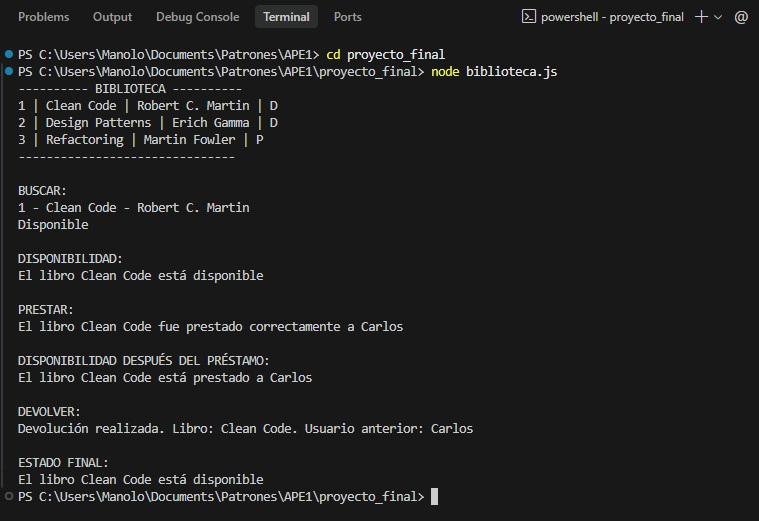
\includegraphics[width=0.9\textwidth]{images/codigofuncional.jpg}
\caption{Ejecuci\'on exitosa del c\'odigo refactorizado en consola. Esta captura evidencia que, tras aplicar todos los principios de Clean Code, SRP y separar la arquitectura en m\'odulos, el sistema de la biblioteca logra procesar exitosamente b\'usquedas, pr\'estamos y devoluciones sin alterar su comportamiento ni arrojar errores.}
\end{figure}
\vspace{8pt}
\textbf{Actividad 8: Control de versiones con Git}

\vspace{4pt}
El proyecto se gestion\'o bajo un repositorio local (\texttt{git init}). Se utiliz\'o un flujo de trabajo iterativo utilizando \texttt{git add .} y \texttt{git commit} con mensajes sem\'anticos convencionales (\texttt{feat}, \texttt{refactor}, \texttt{test}). La evidencia del historial de cambios generada con \texttt{git log} se adjunta detalladamente en el \textbf{Anexo B} de este documento.

\vspace{8pt}
\textbf{Actividad 9: Comparaci\'on antes y despu\'es}

\vspace{4pt}
\begin{table}[H]
\centering
\scriptsize
\renewcommand{\arraystretch}{1.4}
\begin{tabular}{|c|p{2.5cm}|p{2.5cm}|p{2.5cm}|p{3.5cm}|}
\hline
\textbf{N.\textdegree} & \textbf{Problema inicial} & \textbf{Principio aplicado} & \textbf{Refactorizaci\'on} & \textbf{Mejora obtenida} \\
\hline
1 & M\'ultiples ciclos \texttt{for} & DRY & Uso de \texttt{.find()} y \texttt{.filter()} & Iteraciones centralizadas y reutilizables. \\
\hline
2 & \texttt{if/else} anidados & KISS & Retornos tempranos & C\'odigo plano y f\'acil de seguir. \\
\hline
3 & \texttt{var}, nombres ambiguos & Clean Code & \texttt{const}/\texttt{let}, nombres claros & C\'odigo autodocumentado. \\
\hline
4 & Strings "D" y "P" & Clean Code / DRY & Uso de Constantes & Prevenci\'on de errores tipogr\'aficos. \\
\hline
5 & Archivo de 200 l\'ineas & Modularidad & Divisi\'on en 4 directorios & Sistema escalable y ordenado. \\
\hline
6 & Funciones hac\'ian de todo & SRP & Extracci\'on de responsabilidades & L\'ogica independiente de la interfaz. \\
\hline
\end{tabular}
\end{table}

\vspace{12pt}
\textbf{Actividad 10: Documentaci\'on - README.md (Manolo)}

\vspace{4pt}
Se elabor\'o el archivo \texttt{README.md} y se ubic\'o en la ra\'iz del repositorio. Este archivo incluye la descripci\'on del proyecto, los requisitos previos (Node.js), las instrucciones detalladas de instalaci\'on y ejecuci\'on, el \'arbol de carpetas propuesto para la arquitectura final y un resumen de las funcionalidades, adem\'as de las conclusiones t\'ecnicas y principios aplicados en la refactorizaci\'on.

\end{adjustwidth}

\vspace{6pt}

% =============================================================
%  2.8 HABILIDADES BLANDAS
% =============================================================
\begin{adjustwidth}{1.27cm}{0pt}
\textbf{2.8\enspace Habilidades blandas empleadas en la pr\'actica}
\end{adjustwidth}

\vspace{4pt}
\begin{adjustwidth}{0.64cm}{0pt}
$\square$ \; Liderazgo\\[2pt]
$\blacksquare$ \; Trabajo en equipo\\[2pt]
$\blacksquare$ \; Comunicaci\'on asertiva\\[2pt]
$\square$ \; La empat\'ia\\[2pt]
$\blacksquare$ \; Pensamiento cr\'itico\\[2pt]
$\square$ \; Flexibilidad\\[2pt]
$\blacksquare$ \; La resoluci\'on de conflictos\\[2pt]
$\square$ \; Adaptabilidad\\[2pt]
$\blacksquare$ \; Responsabilidad
\end{adjustwidth}

\vspace{6pt}

% =============================================================
%  2.9 CONCLUSIONES
% =============================================================
\begin{adjustwidth}{1.27cm}{0pt}
\textbf{2.9\enspace Conclusiones}
\end{adjustwidth}

\vspace{2pt}
\begin{adjustwidth}{0.64cm}{0pt}
\begin{itemize}[leftmargin=1.27cm, label=\textbullet, topsep=1pt, itemsep=0pt, parsep=0pt]
  \item La detecci\'on temprana de \textit{code smells} es crucial; el c\'odigo monol\'itico analizado demostr\'o c\'omo la falta de encapsulamiento dificulta la comprensi\'on y extensi\'on del sistema.
  \item La aplicaci\'on de Clean Code no solo reduce el n\'umero de l\'ineas, sino que mediante el uso de constantes y nombres sem\'anticos, convierte el c\'odigo en una herramienta autodocumentada \cite{martin2009clean}.
  \item La integraci\'on de los principios DRY y KISS (mediante el uso de cl\'ausulas guarda y funciones de orden superior como \texttt{.find()}) logr\'o reducir dram\'aticamente la complejidad ciclom\'atica, facilitando futuras implementaciones de pruebas unitarias \cite{gamma1994design}.
\end{itemize}
\end{adjustwidth}

\vspace{6pt}

% =============================================================
%  2.10 RECOMENDACIONES
% =============================================================
\begin{adjustwidth}{1.27cm}{0pt}
\textbf{2.10\enspace Recomendaciones}
\end{adjustwidth}

\vspace{2pt}
\begin{adjustwidth}{0.64cm}{0pt}
\begin{itemize}[leftmargin=1.27cm, label=\textbullet, topsep=1pt, itemsep=0pt, parsep=0pt]
  \item Se recomienda integrar un linter (como ESLint) en las etapas iniciales del desarrollo para prevenir la aparici\'on de \textit{code smells} como comparaciones no estrictas o uso de variables globales.
  \item Es aconsejable separar siempre la l\'ogica de negocio de la l\'ogica de presentaci\'on por consola, adhiri\'endose al Principio de Responsabilidad \'Unica (SRP).
  \item Se sugiere mantener el uso de funciones flecha y m\'etodos funcionales de arrays en ECMAScript 6+ para preservar la inmutabilidad y legibilidad de las iteraciones.
\end{itemize}
\end{adjustwidth}

\vspace{6pt}

% =============================================================
%  2.11 REFERENCIAS BIBLIOGRAFICAS
% =============================================================
\begin{adjustwidth}{1.27cm}{0pt}
\textbf{2.11\enspace Referencias bibliogr\'aficas}
\end{adjustwidth}

\vspace{2pt}
\begin{adjustwidth}{0.64cm}{0pt}
\renewcommand{\refname}{\vspace{-4ex}}
\bibliographystyle{ieeetr}
\bibliography{referencias}
\end{adjustwidth}

\vspace{6pt}

% =============================================================
%  2.12 ANEXOS
% =============================================================
\begin{adjustwidth}{1.27cm}{0pt}
\textbf{2.12\enspace Anexos}
\end{adjustwidth}

\vspace{4pt}
\begin{adjustwidth}{0.64cm}{0pt}
\textbf{Anexo A: Arquitectura Propuesta del Sistema Refactorizado}

\begin{lstlisting}[frame=single, numbers=none]
/
|-- models/
|   -- Book.js           # Define la entidad Libro y sus constantes
|-- repositories/
|   -- bookRepository.js # Encargado de la persistencia
|-- services/
|   -- libraryService.js # Lógica de negocio principal
|-- utils/
|   -- formatter.js      # Utilidades de formato
-- biblioteca.js         # Entry point
\end{lstlisting}

\vspace{10pt}
\textbf{Anexo B: Historial de Control de Versiones (Git)}

\vspace{4pt}
El c\'odigo fuente completo, incluyendo la nueva estructura modular y la documentaci\'on asociada, as\'i como el historial detallado de cambios de Git, se encuentran alojados y disponibles de manera p\'ublica en el siguiente repositorio:

\begin{center}
\texttt{https://github.com/Garcia2501/APE1-Biblioteca}
\end{center}

\vspace{4pt}
\begin{table}[H]
\centering
\small
\renewcommand{\arraystretch}{1.2}
\begin{tabularx}{\linewidth}{|l|c|X|}
\hline
\textbf{Fecha} & \textbf{Autor} & \textbf{Mensaje de Commit (Semántico)} \\
\hline
2026-09-01 & Manolo & \texttt{docs: add README.md with instructions} \\
\hline
2026-09-01 & Kevin & \texttt{refactor: extract search logic using .find()} \\
\hline
2026-09-01 & Robert & \texttt{test: add unit tests for libraryService} \\
\hline
2026-09-01 & Kevin & \texttt{style: convert magic strings to constants} \\
\hline
2026-08-30 & Manolo & \texttt{feat: initial commit of legacy system} \\
\hline
\end{tabularx}
\end{table}

\vspace{10pt}
\textbf{Evidencias del Flujo de Trabajo en Git Bash}

\begin{figure}[H]
\centering
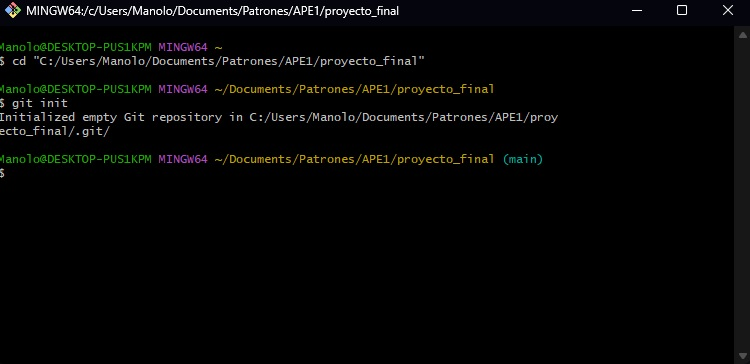
\includegraphics[width=0.85\textwidth]{images/IncioRepo.jpg}
\caption{Inicializaci\'on del repositorio y conexi\'on con GitHub. En esta captura se observa la creaci\'on del repositorio vac\'io en la plataforma GitHub y la configuraci\'on inicial en la terminal local usando Git Bash para vincular el entorno de trabajo con el servidor remoto, estableciendo as\'i la base para el control de versiones.}
\end{figure}

\begin{figure}[H]
\centering
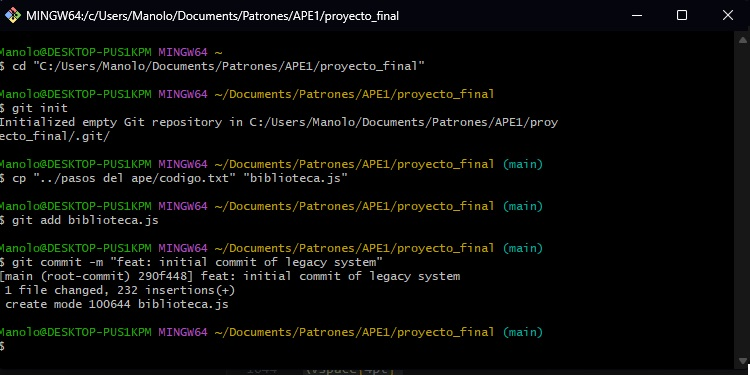
\includegraphics[width=0.85\textwidth]{images/PrimerCommit.jpg}
\caption{Primer commit: Integraci\'on del c\'odigo base (legacy system). Este hito representa el estado original del sistema de biblioteca (\texttt{codigo.txt}) antes de aplicar cualquier refactorizaci\'on. Sirve como punto de partida para que los dem\'as integrantes del equipo puedan comparar el avance t\'ecnico y auditar los cambios.}
\end{figure}

\begin{figure}[H]
\centering
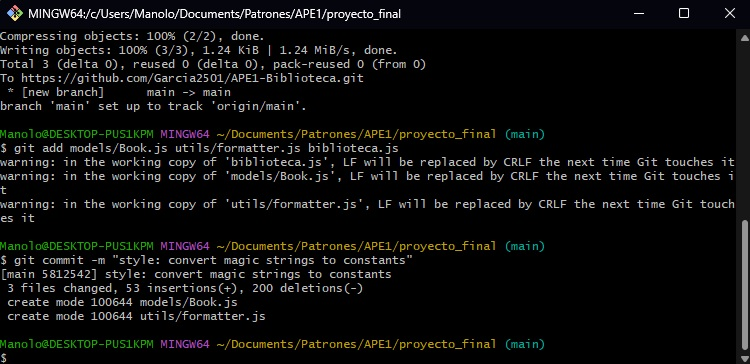
\includegraphics[width=0.85\textwidth]{images/segundoCommit.jpg}
\caption{Segundo commit: Reemplazo de strings m\'agicos por constantes (Clean Code). Se evidencia la modificaci\'on en los archivos del modelo para introducir variables inmutables para los estados de los libros (\texttt{ESTADO\_DISPONIBLE} y \texttt{ESTADO\_PRESTADO}), previniendo as\'i errores de tipograf\'ia y acoplamiento excesivo.}
\end{figure}

\begin{figure}[H]
\centering
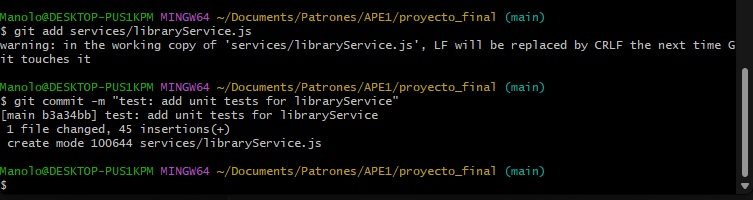
\includegraphics[width=0.85\textwidth]{images/tercerCommit.jpg}
\caption{Tercer commit: Implementaci\'on de servicios y pruebas manuales. Muestra la introducci\'on de la l\'ogica de negocio para las funciones de pr\'estamo y devoluci\'on, aplicando intensivamente el principio KISS mediante cl\'ausulas guarda (\textit{early returns}) para simplificar la profundidad de anidamiento condicional.}
\end{figure}

\begin{figure}[H]
\centering
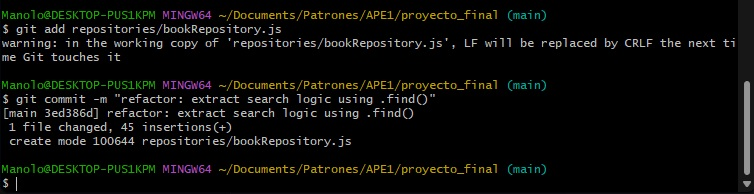
\includegraphics[width=0.85\textwidth]{images/cuartoCommit.jpg}
\caption{Cuarto commit: Centralizaci\'on de la b\'usqueda usando arreglos iterativos (DRY). En esta etapa de la refactorizaci\'on se eliminaron los m\'ultiples bucles \texttt{for} repetitivos, delegando el algoritmo de b\'usqueda de libros hacia m\'etodos funcionales de alto orden como \texttt{.find()} y \texttt{.filter()} en el repositorio de datos.}
\end{figure}

\begin{figure}[H]
\centering
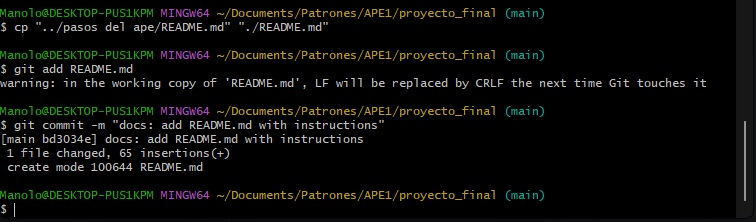
\includegraphics[width=0.85\textwidth]{images/commitReadme.jpg}
\caption{Quinto commit: Integraci\'on del archivo README.md al ecosistema del proyecto. Se agrega formalmente el archivo de documentaci\'on principal que instruye a los desarrolladores c\'omo instalar, desplegar y probar el sistema localmente, dotando al repositorio de gran autonom\'ia formativa.}
\end{figure}

\begin{figure}[H]
\centering

\includegraphics[width=0.85\textwidth]{images/pushfinal.jpg}
\caption{Subida final (push) del historial local consolidado hacia la rama main del servidor remoto. Esta acci\'on de red confirma la sincronizaci\'on exitosa y segura de la totalidad de los \textit{commits} y el c\'odigo fuente de la biblioteca refactorizada, concluyendo as\'i con el flujo del trabajo colaborativo.}
\end{figure}
\end{adjustwidth}

\end{document}

